\documentclass{Interspeech}
\usepackage[T1]{fontenc}
\usepackage{tabularx}
\usepackage{microtype}
\newcommand{\model}{OFA-TS\xspace}
\newcommand{\bench}{AmphionTS-Bench\xspace}
\newcommand{\sepvec}{\mathbf{s}}
\title{OFA-TS: One Model for All Real-World Scenarios\\in Target-Speaker ASR}
\author{Amphion}{Team}
\address{}
\email{}
\keywords{target-speaker speech recognition, real-world scenarios, unified model, false alarms}

\begin{document}
\maketitle
\begin{abstract}
Target-speaker ASR must recognize an enrolled speaker across changing acoustic and conversational conditions and remain silent when the target is absent.
We present OFA-TS, a single model for noisy and far-field speech, multi-speaker interactions, short utterances, and target absence.
Initialized from Qwen3-ASR-1.7B, it joins enrollment and mixture features inside the audio encoder and trains with target-absent counterparts across scene types.
We evaluate the same weights on AmphionTS-Bench, with 24,101 Mandarin samples in 248 subsets spanning synthetic conditions and real meetings, calls, and web conversations.
OFA-TS achieves 13.1\% character error rate with the target present and 3.7\% false-alarm rate with the target absent, versus 33.4\% and 67.8\% for Xiaomi-CocktailASR-1.
Paired diagnostics identify short similar-sounding speech as a remaining weakness.

\end{abstract}
% Condensed from the source report, Sections 1 and 7.
\section{Introduction}
\label{sec:introduction}
Across meetings, phone calls, and continuously listening applications, a recognizer may need to transcribe one person despite changes in acoustics and speaker activity.
Target-speaker automatic speech recognition (TS-ASR) receives a short enrollment recording of that person and a recording to transcribe, called the mixture.
It must recognize the target's words despite competing voices, but also return an empty transcript when only other people speak.
A system that recognizes speech accurately yet frequently transcribes the wrong person fails this task.

Common evaluations such as WSJ0-2mix, LibriMix, and LibriSpeechMix overlay read utterances and assume that the target is present~\cite{hershey2016deep,cosentino2020librimix,kanda2020serialized}.
They measure recognition or separation under overlap, but cannot expose false alarms when the enrolled speaker is absent.
Prior target speech extraction work has studied this failure explicitly~\cite{delcroix2022listen,borsdorf2021universal,zhang2023speaker}.
Enrollment-conditioned speech models, including SQ-Whisper and CocktailASR, extend recognition to competing speakers~\cite{guo2024sqwhisper,zhang2025thinking,zhang2026xiaomi}.
Real meeting benchmarks address speaker-attributed transcription~\cite{liang2023second,vinnikov2024notsofar}, but this differs from recognizing a single enrolled person and rejecting all others.
The remaining evaluation gap is to test both behaviors across conversational timing, degraded enrollment, and real recordings.

We introduce \model (One For All Target-Speaker ASR), using the same model parameters across noise, reverberation, turn-taking, overlap, short utterances, and target absence.
It builds on Qwen3-ASR-1.7B~\cite{shi2026qwen3asr}, conditions its audio encoder on enrollment speech, and trains with target-absent counterparts across scene types.
This extends the speaker-selection capability studied in AmphionASR~1.0~\cite{amphion2026amphionasr}.
To evaluate this scenario coverage, we introduce \bench, with 24{,}101 Mandarin samples in 248 subsets.
It combines controlled synthetic conditions with real meetings, telephone calls, and web conversations, measuring recognition, complete misses, and false alarms together.

The benchmark changes how systems compare.
When only the target speaks in real recordings, \model and Xiaomi-CocktailASR-1 have nearly identical character error rates (CERs), 7.5\% and 7.3\%.
When others speak while the target is absent, their false-alarm rates are 2.6\% and 96.1\%.
This contrast motivates evaluating target absence as a distinct requirement rather than treating silence-only tests as sufficient.

% Source: sections/02_benchmark.tex and its composition/metric definitions.
\section{AmphionTS-Bench}
\label{sec:benchmark}
We evaluate one model across the conditions in Table~\ref{tab:composition}, with 12{,}950 target-present and 11{,}151 target-absent samples.
The benchmark's synthetic part has 21{,}720 samples; 2{,}381 come from real recordings.
The benchmark is intended for public release.

\begin{table}[t]
\caption{Benchmark composition. P/A: target present/absent. Counts include diagnostic subsets.}
\label{tab:composition}
\centering
\small
\begin{tabularx}{\columnwidth}{@{}Xrrr@{}}
\toprule
Condition & Subsets & P & A \\
\midrule
Degraded enrollment & 22 & 1{,}650 & 1{,}650 \\
Timing and interferers & 27 & 2{,}280 & 960 \\
Short segments & 15 & 2{,}520 & 1{,}080 \\
No one speaking & 10 & 0 & 1{,}200 \\
Noise and recording chain & 52 & 3{,}240 & 3{,}000 \\
Far field and reverberation & 22 & 1{,}320 & 1{,}320 \\
Real conversations & 88 & 1{,}190 & 1{,}191 \\
Additional diagnostics & 12 & 750 & 750 \\
\midrule
Total & 248 & 12{,}950 & 11{,}151 \\
\bottomrule
\end{tabularx}
\end{table}

\subsection{Paired synthetic conditions}
Synthetic speech comes from the official test splits of AISHELL-1/2/3, KeSpeech, and MagicData~\cite{bu2017aishell1,du2018aishell2,shi2021aishell3,tang2021kespeech}.
Scenes cover turn-taking, simultaneous starts, interruptions, the target entering or leaving, short replies, and multiple interferers.
Enrollment degradations include limited speech, leading silence, narrowband audio, noise, reverberation, and another voice.
Other subsets vary noise floors, room responses, recording level, and background sounds, including music and babble without a target.

Controlled comparisons change one factor on the same base scenes.
For paired target-absent samples, the mixture remains identical while the enrollment changes to another person.
This person is either random or among the five speakers whose embeddings are closest to an interferer.
The similar-voice condition tests a failure that random enrollment alone can hide.
Each enrollment stores 10\,s; evaluation uses its first 5\,s, with zero-padding when shorter.
Separate subsets test enrollments recorded for only 2--4\,s.

\subsection{Real recordings and label checks}
Real samples are sentence-aligned windows from AliMeeting and AISHELL-4 far-field meetings~\cite{yu2022m2met,fu2021aishell4}, MagicData-RAMC calls~\cite{yang2022open}, and Emilia web conversations~\cite{he2024emilia}, without synthetic mixing.
The first three use human-annotated test sets; web conversations use pseudo-labels.
Present samples enroll someone who speaks for at least 1\,s in the window.
Absent samples enroll a silent participant from the same recording, or a speaker from another recording of the same corpus when necessary.
Enrollment speech is taken outside the window with a 1\,s margin.

Speaker embeddings are used to check enrollment identity.
Three mismatched AISHELL-4 enrollments were replaced and one unconfirmed window removed.
Enrollments containing at least 0.3\,s of another voice in their first 5\,s are evaluated separately.
AliMeeting also provides paired near-field and far-field conditions to compare synthetic degradation with real microphone mismatch.

\subsection{English counterpart}
An English counterpart uses the same synthetic recipe and random seed, with speech from VCTK, the English test portion of CS-Dialogue, and LibriSpeech test-clean and test-other~\cite{yamagishi2019cstr,zhou2025csdialogue,panayotov2015librispeech}.
Its synthetic and diagnostic subsets match Table~\ref{tab:composition} in number and size.
Its real section has 60 subsets with 661 target-present and 640 target-absent samples, giving 220 subsets and 23{,}021 samples.
Real windows come from human-annotated test or evaluation sessions of AMI, NOTSOFAR-1, CHiME-6, DiPCo, and ICSI~\cite{carletta2005ami,vinnikov2024notsofar,watanabe2020chime6,vansegbroeck2019dipco,janin2003icsi}; ICSI uses the close-talk headset mix rather than a distant microphone.
Enrollment again comes from the same person outside the window, and enrollments containing another voice are evaluated separately.

\subsection{Metrics}
Mandarin text is converted to simplified characters, numbers are normalized, and filler words are removed; English text uses the Whisper English normalizer~\cite{radford2023robust}.
CER pools character errors and reference characters over target-present samples; English uses the word error rate (WER) in the same way.
The empty-output rate (ER) is the fraction of target-present samples with an empty normalized transcript.
The false-alarm rate (FA) is the fraction of target-absent samples with a nonempty normalized transcript.
These metrics must be read together: suppressing every output reduces FA but increases ER.
Section and overall scores are pooled over their constituent samples, rather than averaged across subsets.

% Source: sections/03_model.tex, 04_data.tex and 05_training.tex.
\section{OFA-TS: model and training}
\label{sec:model}
\subsection{Enrollment inside the audio encoder}
\model initializes both its audio encoder and language model from Qwen3-ASR-1.7B~\cite{shi2026qwen3asr}.
The AuT encoder has convolutional downsampling and a 24-layer Transformer.
It maps 128-dimensional Mel features from 16\,kHz mono audio to 12.5\,Hz embeddings.
The language model has 1.7\,B parameters; including the approximately 300\,M encoder, the total is about 2.0\,B.

Figure~\ref{fig:model} shows the TS-ASR input.
Enrollment and mixture features pass separately through the shared convolutional downsampling, preventing a convolutional receptive field from crossing their boundary.
Their output sequences, $H_e$ and $H_x$, are then joined by a trainable 1024-dimensional separator $\sepvec$:
\begin{equation}
H = [H_e;\,\sepvec;\,H_x].
\label{eq:input}
\end{equation}
The Transformer uses one attention window over the entire sequence, so every mixture frame can attend to the enrollment.
Projected encoder outputs and a fixed task instruction enter the language model.
The output language tag carries the presence decision: a present target is followed by its transcript, whereas absence yields no language and an empty transcript.
A request contains at most 30\,s of audio; the default 5\,s enrollment leaves at most 25\,s for the mixture.

\begin{figure}[t]
\centering
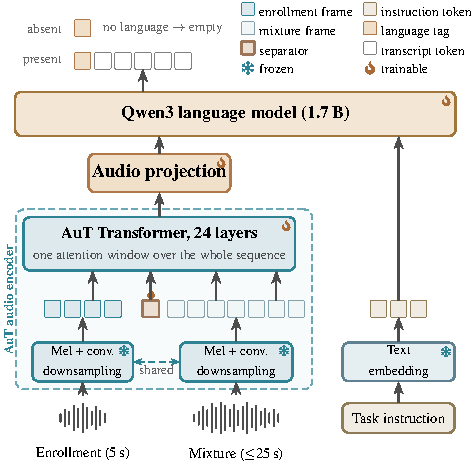
\includegraphics[width=\columnwidth]{figures/model.pdf}
\caption{OFA-TS architecture in TS-ASR mode, shared across scenarios. Enrollment and mixture pass separately through the same frozen convolutional downsampling. A learnable separator, introduced during fine-tuning, joins the two sequences before the Transformer layers of the audio encoder, which attend over the whole sequence. The LLM reads the projector output and a fixed task instruction, and its output language tag carries the presence decision. Audio encoder and LLM are initialized from Qwen3-ASR-1.7B.}
\label{fig:model}
\end{figure}

% Full-width result tables of Section 4, defined here so that they float to the top of the
% page on which Section 4 begins.
\begin{table*}[t]
\caption{TS-ASR results on the Mandarin benchmark and its English counterpart (\%, lower is better). The error rate is CER in Mandarin and WER in English. Error rate and ER use target-present samples; FA uses target-absent samples. For real recordings, the error rate excludes enrollments that contain another voice, whereas FA includes them. Type: extract-then-recognize cascade or end-to-end (E2E) model. Bold marks the lowest value in each column.}
\label{tab:overall}
\centering
\small
\setlength{\tabcolsep}{3.9pt}
\begin{tabular}{@{}llrrrrrrrrrrrr@{}}
\toprule
 & & \multicolumn{6}{c}{Mandarin} & \multicolumn{6}{c}{English} \\
\cmidrule(lr){3-8}\cmidrule(l){9-14}
 & & \multicolumn{3}{c}{All} & Synthetic & \multicolumn{2}{c}{Real} & \multicolumn{3}{c}{All} & Synthetic & \multicolumn{2}{c}{Real} \\
\cmidrule(lr){3-5}\cmidrule(lr){6-6}\cmidrule(lr){7-8}\cmidrule(lr){9-11}\cmidrule(lr){12-12}\cmidrule(l){13-14}
System & Type & CER & ER & FA & FA & FA & CER & WER & ER & FA & FA & FA & WER \\
\midrule
WeSep + Qwen3-ASR-1.7B & Cascade & 62.0 & \textbf{0.3} & 87.0 & 85.5 & 99.4 & 37.2 & 64.6 & 0.9 & 81.8 & 81.3 & 88.8 & 50.9 \\
LauraTSE + Qwen3-ASR-1.7B & Cascade & 80.5 & 12.6 & 64.9 & 64.2 & 70.4 & 81.2 & 74.6 & 17.3 & 58.7 & 58.7 & 58.0 & 79.3 \\
\midrule
CocktailASR-1 & E2E & 33.4 & 2.7 & 67.8 & 64.4 & 96.1 & 30.8 & 26.3 & 5.0 & 50.6 & 47.5 & 98.0 & 35.2 \\
CocktailASR-1-CoT & E2E & 39.6 & 3.0 & 61.9 & 58.8 & 87.7 & 27.2 & 25.3 & \textbf{0.6} & 61.3 & 58.9 & 97.5 & 31.0 \\
OFA-TS (ours) & E2E & \textbf{13.1} & 3.3 & \textbf{2.8} & \textbf{2.8} & \textbf{2.4} & \textbf{9.2} & \textbf{13.6} & 3.7 & \textbf{6.3} & \textbf{5.5} & \textbf{19.5} & \textbf{15.3} \\
\bottomrule
\end{tabular}
\end{table*}

\begin{table*}[t]
\caption{Selected Mandarin diagnostic subsets (\%, lower is better). Target-present subsets are scored by CER and target-absent subsets by FA. All rows use 5\,s enrollment. Type as in Table~\ref{tab:overall}. Bold marks the lowest value in each column.}
\label{tab:diagnostics}
\centering
\small
\newcommand{\hd}[1]{\begin{tabular}[b]{@{}c@{}}#1\end{tabular}}
\setlength{\tabcolsep}{5pt}
\begin{tabular}{@{}llrrrrrrr@{}}
\toprule
 & & \multicolumn{3}{c}{Target present: CER} & \multicolumn{4}{c}{Target absent: FA} \\
\cmidrule(lr){3-5}\cmidrule(l){6-9}
System & Type & \hd{Target only,\\real\\recordings} & \hd{Target +\\one\\interferer} & \hd{Target +\\2--4\\interferers} & \hd{Nobody\\speaking} & \hd{Others\\speaking,\\synthetic} & \hd{Others\\speaking,\\real} & \hd{Similar-\\sounding\\speaker} \\
\midrule
WeSep + Qwen3-ASR-1.7B & Cascade & \textbf{5.4} & 69.1 & 215.9 & 7.1 & 97.1 & 99.4 & 99.1 \\
LauraTSE + Qwen3-ASR-1.7B & Cascade & 84.3 & 48.0 & 198.7 & 9.0 & 80.8 & 70.4 & 73.7 \\
\midrule
CocktailASR-1 & E2E & 7.3 & 21.3 & 65.7 & 10.8 & 85.8 & 96.1 & 73.9 \\
OFA-TS (ours) & E2E & 7.7 & \textbf{6.8} & \textbf{18.5} & \textbf{0.8} & \textbf{1.7} & \textbf{2.4} & \textbf{13.9} \\
\bottomrule
\end{tabular}
\end{table*}

\subsection{Training with absent counterparts}
Training has two stages.
Three rounds of multi-task supervised fine-tuning use plain ASR, hotword ASR, synthetic target-speaker mixtures, and meeting turn-taking data.
Subsequent robustness-training segments continue from the preceding weights with adjusted data recipes.
% TODO: verify the number of robustness segments behind the evaluated checkpoint
% (ts-robust-064-avg3: 064 <- 062 <- 059 <- 057; the weights 057 started from are not recorded).
All parameters are updated except the encoder convolutions and text embeddings.
The objective is cross-entropy over predicted text positions.
Final weights average the last three checkpoints~\cite{wortsman2022model}.

Robustness training combines online mixtures, constructed conversational scenes, and real meeting windows.
Online mixing varies up to four interferers, signal levels, room responses, noise, and enrollment quality.
Scene pools add turn-taking, hand-overs, and brief target utterances that random overlap does not reproduce.
Every scene type has target-absent counterparts: the scene is retained but another person is enrolled, sometimes with a similar voice, and the reference is empty.
Enrollment that repeats the target sentence is excluded.
Meeting-window labels are checked to remove supposed absent samples in which the target actually speaks.

Target voices come from AISHELL-2, LibriSpeech, KeSpeech, MagicData, and Emilia; conversational sources also include AliMeeting, AISHELL-4, MagicData-RAMC, AMI, CHiME-6, NOTSOFAR-1, DiPCo, and ICSI~\cite{panayotov2015librispeech,carletta2005ami,watanabe2020chime6,vinnikov2024notsofar,vansegbroeck2019dipco,janin2003icsi}.
Noise-only and babble samples have empty reference transcripts.
Plain and hotword ASR data remain in the training mixture.
A small amount of non-public domain speech and meeting-room noise is also used.

% Source: sections/06_experiments.tex (structure). Numbers: AmphionEval records
% (protocol v4) of ts-robust-064-avg3 and of the two CocktailASR-1 modes, pooled over
% the 248 subsets of Table 1 (v12) and the 220 English subsets (en-v1). The English
% CocktailASR-1 predictions were rescored with the same Whisper normalizer version.
% Cascades (WeSep or LauraTSE + Qwen3-ASR-1.7B): full AmphionEval external-worker runs on
% both sets (2026-11-22, same protocol and normalizer), pooled with the same script.
\section{Experiments}
\label{sec:experiments}
\subsection{Protocol and baselines}
We use one set of \model weights across all subsets in both languages, with the first 5\,s of enrollment and the same normalization for all systems.
\model uses greedy decoding with at most 512 output tokens.
The end-to-end (E2E) TS-ASR baseline is CocktailASR-1~\cite{zhang2026xiaomi} in its standard and chain-of-thought modes, denoted CocktailASR-1 and CocktailASR-1-CoT, using the publicly available \texttt{Ease3/Xiaomi-CocktailASR-1} weights and their accompanying inference code with bf16 and greedy decoding, at most 256 output tokens in Mandarin and 512 in English.
Its report evaluates enrollment-conditioned transcription and rejection of absent targets in both Chinese and English.
Baseline scores are measured on the same audio and scoring protocol, not copied from their reports.

We also evaluate two extract-then-recognize cascades.
A target speech extraction (TSE) model receives the same enrollment and the mixture, and Qwen3-ASR-1.7B transcribes its output with greedy decoding.
WeSep~\cite{wang2024wesep} uses its public English BSRNN model with an ECAPA speaker encoder.
LauraTSE~\cite{tang2025lauratse}, a generative extractor built on a decoder-only language model, uses offline inference with top-25 sampling and a fixed seed.
We denote them WeSep + Qwen3-ASR-1.7B and LauraTSE + Qwen3-ASR-1.7B.
Neither cascade has a separate rejection step: an absent target counts as rejected only when the transcript is empty.

The CocktailASR-1 report uses reference crops of 1--4\,s.
On an earlier benchmark version, a fixed 3\,s crop and that random-crop protocol produced similar target-absent FA, although group CER differed by up to about seven points.
Our main comparison holds enrollment length fixed across systems.

\subsection{One model across scenarios}
Table~\ref{tab:overall} reports all three metrics.
In Mandarin, \model achieves 13.1\% CER against 33.4\% for CocktailASR-1, with an ER 0.6 points higher (3.3\% versus 2.7\%).
Thus the lower FA is not explained by a large increase in completely suppressed target utterances.
Overall FA is 2.8\% versus 67.8\%; CocktailASR-1-CoT reduces FA to 61.9\% but increases CER to 39.6\%.
The cascades rarely return empty transcripts.
WeSep + Qwen3-ASR-1.7B has the lowest ER, 0.3\%, but 87.0\% FA and 62.0\% CER; LauraTSE + Qwen3-ASR-1.7B has 64.9\% FA and 80.5\% CER.

On real conversations with clean enrollments, CER is 9.2\% versus 30.8\%.
For individual real corpora with clean enrollments, \model has FA between 1\% and 7\%, compared with 74--100\% for CocktailASR-1.
For example, AliMeeting far-field CER is 6.3\% versus 38.2\%, and FA is 1.0\% versus 100.0\%.
When the enrollment contains another voice, our CER rises from 10.4\% to 15.0\% on AliMeeting, AISHELL-4, and web-conversation windows, and from 7.3\% to 18.6\% on the paired AliMeeting windows; with such enrollments, FA is 0.7\%.
These are whole-system comparisons: the study does not separately establish the contributions of architecture, training data, or parameter count.

\subsection{What restricted evaluations miss}
Table~\ref{tab:diagnostics} contrasts common evaluation conditions with cases encountered during continuous listening.
Single-talker real recordings barely distinguish the systems.
Adding silence-only negatives gives CocktailASR-1 a 10.8\% FA, while negatives containing other speakers reveal much higher FA.
With two to four interferers and the target present, its CER reaches 65.7\%, versus 18.5\% for \model.
Both target presence and conversation structure therefore affect the comparison.
The cascades follow the same pattern more strongly.
On single-talker real recordings, WeSep + Qwen3-ASR-1.7B has the lowest CER, 5.4\%, but with two to four interferers both cascades exceed 190\% CER, and with only others speaking their FA is 70--99\%.

Paired enrollment tests expose a remaining weakness.
For 6--18\,s absent-target segments, replacing a random enrollment with a similar-sounding person's enrollment raises our FA from 0.0\% to 10.8\%.
For a single short phrase, it rises from 3.0\% to 16.7\%.
Only 1\,s of enrollment speech also raises FA to 18.0\%.
Short, similar voices remain difficult despite the low overall FA.

Real near/far-field pairs qualify synthetic robustness conclusions.
With near-field enrollment, switching the mixture to far field increases our CER from 9.4\% to 18.9\% synthetically, but from 4.6\% to 7.6\% on the paired AliMeeting windows.
Synthetic subsets identify sensitivity; real windows measure its magnitude under actual recording conditions.

\subsection{English counterpart}
The English columns of Table~\ref{tab:overall} apply the same protocol to the English counterpart.
\model has 13.6\% WER against 26.3\% for CocktailASR-1, and an ER of 3.7\% against 5.0\%; CocktailASR-1-CoT has the lowest ER, 0.6\%.
FA is 6.3\% versus 50.6\%, and 81.8\% and 58.7\% for WeSep + Qwen3-ASR-1.7B and LauraTSE + Qwen3-ASR-1.7B.
With similar-sounding absent speakers, our FA is 20.2\%, against 13.9\% in Mandarin.

Real English conversations are harder than Mandarin ones: FA is 19.5\%, against 2.4\% in Mandarin.
With clean enrollments, our FA ranges from 2.4\% on ICSI and 5.2\% on NOTSOFAR-1 to 28.6\% on DiPCo and 69.3\% on CHiME-6, while CocktailASR-1 has 92.7--100\% on every corpus.

\subsection{Limitations}
Both language versions are mostly synthetic, and the English real section has only 1{,}301 samples.
Real data cover meetings, calls, and web conversations; web references contain pseudo-label errors.
Training uses the training splits of the Mandarin real meeting corpora and also includes recordings from all five English real corpora, so the real results measure in-domain behavior.
The same team designed training scenes and benchmark conditions.
AISHELL-1 test text overlaps with AISHELL-2 training text, and MagicData-RAMC speaker-ID inconsistencies may allow speaker overlap.
The benchmark therefore does not establish unseen-domain or fully speaker-disjoint generalization.
There is no controlled architectural ablation or formal significance test.
The cascades use public extraction checkpoints trained on LibriSpeech-based mixtures (LauraTSE) and VoxCeleb (WeSep)~\cite{tang2025lauratse}, without adaptation to Mandarin or to our training data; they compare available systems, not extraction as an approach.
An empty transcript is not an identity guarantee, and recordings longer than the request limit require segmentation.

% Source: sections/09_conclusion.tex; no new experimental claims.
\section{Conclusion}
\label{sec:conclusion}
\model uses one model across diverse acoustic and conversational scenarios, combining enrollment-conditioned encoder attention with training that covers target absence in each scene type.
\bench evaluates this coverage through paired conditions and real recordings.
Under the matched protocol, \model reduces both target-present CER and target-absent false alarms against CocktailASR-1.
Short similar-sounding voices and the benchmark's Mandarin coverage remain limitations.
Testing both target presence and absence is essential to assess recognition across scenarios.

\section{Generative AI Use Disclosure}
Generative AI tools assisted in drafting the source technical report and in condensing and editing this conference version. Numerical results are pooled from existing evaluation records of the reported checkpoint; no new experiments were performed for this adaptation.
\bibliographystyle{IEEEtran}
\bibliography{references}
\end{document}
